%%%%%%%%%%%%%%%%%%%%%%%%%%%%%%%%%%%%%%%%%%%%%%%%%%%%%%%%%%%%%%%%%%%%%%%%%%%%%%%%
%2345678901234567890123456789012345678901234567890123456789012345678901234567890
%        1         2         3         4         5         6         7         8

%\documentclass[journal,transmag]{IEEEtran}% Comment this line out if you need a4paper

\documentclass[10pt, conference]{ieeeconf}      % Use this line for a4 paper


\IEEEoverridecommandlockouts                              % This command is only needed if 
                                                          % you want to use the \thanks command

%\overrideIEEEmargins                                      % Needed to meet printer requirements.

% See the \addtolength command later in the file to balance the column lengths
% on the last page of the document

% The following packages can be found on http:\\www.ctan.org
%\usepackage{graphics} % for pdf, bitmapped graphics files
%\usepackage{epsfig} % for postscript graphics files
%\usepackage{mathptmx} % assumes new font selection scheme installed
%\usepackage{times} % assumes new font selection scheme installed
%\usepackage{amsmath} % assumes amsmath package installed
%\usepackage{amssymb}  % assumes amsmath package installed

\newtheorem{theorem}{Theorem}[section]
\newtheorem{lemma}[theorem]{Lemma}
\newtheorem{proposition}[theorem]{Proposition}
\newtheorem{corollary}[theorem]{Corollary}
\usepackage[ruled,vlined]{algorithm2e}
\usepackage{url}
\newenvironment{definition}[1][Definition]{\begin{trivlist}
\item[\hskip \labelsep {\bfseries #1}]}{\end{trivlist}}

\newcommand{\qed}{\nobreak \ifvmode \relax \else
      \ifdim\lastskip<1.5em \hskip-\lastskip
      \hskip1.5em plus0em minus0.5em \fi \nobreak
      \vrule height0.75em width0.5em depth0.25em\fi}

\def\lc{\left\lfloor}   
\def\rc{\right\rfloor}

\usepackage{amsmath,amssymb}

\usepackage{tabularx}
\usepackage{tikz,hyperref,graphicx,units}
\usepackage{subfigure}
\usepackage{benktools}
\usepackage{bbm}
\renewcommand{\baselinestretch}{.5}

\usepackage{caption}
\usepackage{epstopdf}
\renewcommand{\captionfont}{\footnotesize}
\usepackage{sidecap,wrapfig}
\usepackage[ruled,vlined]{algorithm2e}
\DeclareMathOperator*{\argmin}{arg\,min}
\DeclareMathOperator*{\argmax}{arg\,max}
\newcommand{\abs}[1]{\lvert#1\rvert} 
\newcommand{\norm}[1]{\lVert#1\rVert}
%\newcommand{\suchthat}{\mid}
\newcommand{\suchthat}{\ \big|\ }
\newcommand{\ba}{\mathbf{a}}
\newcommand{\bb}{\mathbf{b}}
\newcommand{\bc}{\mathbf{c}}
\newcommand{\bd}{\mathbf{d}}
\newcommand{\bg}{\mathbf{g}}
\newcommand{\bj}{\mathbf{j}}
\newcommand{\bn}{\mathbf{n}}
\newcommand{\bp}{\mathbf{p}}
\newcommand{\bw}{\mathbf{w}}
\newcommand{\bt}{\mathbf{t}}
\newcommand{\bu}{\mathbf{u}}
\newcommand{\by}{\mathbf{y}}
\newcommand{\bx}{\mathbf{x}}
\newcommand{\bz}{\mathbf{z}}
\newcommand{\bbf}{\mathbf{f}}
\newcommand{\bzero}{\mathbf{0}}
\newcommand{\bG}{\mathbf{G}}
\newcommand{\bA}{\mathbf{A}}
\newcommand{\bW}{\mathbf{W}}
\newcommand{\bX}{\mathbf{X}}
\newcommand{\mX}{\mathcal{X}}
\newcommand{\mD}{\mathcal{D}}
\newcommand{\mG}{\mathcal{G}}
\newcommand{\mN}{\mathcal{N}}
\newcommand{\mW}{\mathcal{W}}
\newcommand{\mF}{\mathcal{F}}
\newcommand{\bZ}{\mathbf{Z}}
\newcommand{\mR}{\mathcal{R}}

\newcommand{\bfc}{W}
\newcommand{\Qinf}{Q_{\infty}}
\newcommand{\st}[1]{_\text{#1}}
\newcommand{\rres}{r\st{res}}
\newcommand{\pos}[1]{(#1)^+}
\newcommand{\depth}{\operatorname{depth}}
\newcommand{\dist}{\operatorname{dist}}
\newcommand{\convhull}{\operatorname{ConvexHull}}
\newcommand{\minksum}{\operatorname{MinkowskiSum}}

\newcommand{\specialcell}[2][c]{ \begin{tabular}[#1]{@{}c@{}}#2\end{tabular}}
\newcommand{\acro}{SHIV}
\newcommand\independent{\protect\mathpalette{\protect\independenT}{\perp}}
\def\independenT#1#2{\mathrel{\rlap{$#1#2$}\mkern2mu{#1#2}}}

\newcolumntype{L}[1]{>{\RaggedRight\hspace{0pt}}p{#1}}
\newcolumntype{R}[1]{>{\RaggedLeft\hspace{0pt}}p{#1}}


\newboolean{include-notes}
\setboolean{include-notes}{true}
\newcommand{\adnote}[1]{\ifthenelse{ \boolean{include-notes}}%
 {\textcolor{blue}{\textbf{AD: #1}}}{}}
 
 \newcommand{\fpnote}[1]{\ifthenelse{ \boolean{include-notes}}%
 {\textcolor{blue}{\textbf{FP: #1}}}{}}
 
  \newcommand{\mlnote}[1]{\ifthenelse{ \boolean{include-notes}}%
 {\textcolor{purple}{\textbf{ML: #1}}}{}}

\renewcommand{\baselinestretch}{.95}
\usepackage{times}
\usepackage{microtype}
%\title{Iterative Imitation Learning with Reduced Human Supervision [v11]}
%\title{SHIV:  Reducing Human Supervision for Robot Active Learning [v11]}

\title{Robot Grasping in Clutter:\\
 Using a Hierarchy of Supervisors for Learning from Demonstrations}



\author{Michael Laskey$^1$, Jonathan Lee$^1$, Caleb Chuck$^1$, David Gealy$^1$, Wesley Hsieh$^1$, Florian T. Pokorny$^1$,\\
 Anca D. Dragan$^1$, and Ken Goldberg$^{1,2}$% <-this % stops a space
\thanks{$^1$ Department of Electrical Engineering and Computer Sciences; {\small \{mdlaskey, jonathan\textunderscore lee, calebchuck, dgealy, wesleyhsieh, ftpokorny, anca\}@berkeley.edu} }%
\thanks{$^2$ Department of Industrial Engineering and Operations Research; {\small goldberg@berkeley.edu}}%
\thanks{$^{1-2}$ University of California, Berkeley;  Berkeley, CA 94720, USA}%
}
\begin{document}



\maketitle
\thispagestyle{empty}
\pagestyle{empty}


%%%%%%%%%%%%%%%%%%%%%%%%%%%%%%%%%%%%%%%%%%%%%%%%%%%%%%%%%%%%%%%%%%%%%%%%%%%%%%%%

\begin{abstract}
For applications such as Amazon warehouse order fulfillment, robots must grasp a desired object amid clutter: other objects that block direct access. This can be difficult to program explicitly due to uncertainty in friction and push mechanics and the variety of objects that can be encountered. Deep Learning networks combined with Online Learning from Demonstration (LfD) algorithms such as DAgger and SHIV have potential to learn robot control policies for such tasks where the input is a camera image and system dynamics and the cost function are unknown.  To explore this idea, we introduce a version of the grasping in clutter problem where a yellow cylinder must be grasped by a planar robot arm amid extruded objects in a variety of shapes and positions. To reduce the burden on human experts to provide demonstrations, we propose using a hierarchy of three levels of supervisors: a fast motion planner that ignores obstacles, crowd-sourced human workers who provide appropriate robot control values remotely via online videos, and a local human expert. Physical experiments suggest that with a fixed budget of 160 expert demonstrations, using the hierarchy of supervisors can increase the probability of a successful grasp (reliability) from $55\%$ to $90\%$.

 \end{abstract}


%%%%%%%%%%%%%%%%%%%%%%%%%%%%%%%%%%%%%%%%%%%%%%%%%%%%%%%%%%%%%%%%%%%%%%%%%%%%%%%%

\section{Introduction} 
As illustrated by the recent Amazon Picking Challenge at ICRA 2015, the grasping in clutter problem, where a robot needs
to grasp an object that might be occluded by other objects in the environment poses an interesting challenge to robotic
systems. This problem is relevant to industrial applications such as warehouse shipping operations and flexible manufacturing in semi-structured environments. One fundamental approach to grasping in clutter is the analytic model driven approach~\cite{bicchi2000robotic},
where the interaction dynamics between the robot and obstacles are formulated analytically. However, modeling all the 
physical properties of interaction poses a highly challenging problem due to uncertainty in modeling parameters such as
inertial properties and friction. 

Another approach to the grasping in
clutter problem is a data-driven manner, where the interaction behavior is learned directly from interactions with the environment and a supervisor, which can be an expert human or an analytical method \cite{argall2009survey}. Learning from demonstration (LfD) algorithms have been used
successfully in recent years for a large number of robotic tasks, including helicopter
maneuvering~\cite{abbeel2007application}, car parking~\cite{abbeel2008apprenticeship},  and robot
surgery~\cite{van2010superhuman}. Furthermore, deep learning, which we use to learn policies directly from raw video
data, has emerged as a highly versatile technique used for this purpose ~\cite{pinto2015supersizing}.

\begin{figure}
\includegraphics[width=0.5\textwidth]{f_figs/teaser_h.eps}
\caption{
    \footnotesize
Three policy roll-outs on a Zymark 3-DOF Robot of a fully trained grasping in clutter policy (one per row, left to
right) which was trained using a hierarchy of three supervisors consisting of a motion planning algorithm, crowd-sourcing and a human expert. 
Red shapes indicate clutter objects and the robot is trained to reach the yellow cylinder. The trained manipulation
policy is represented as a deep neural network that receives as input an image of the scene and outputs a change in
state position. The resulting policy learns to sweep away clutter objects to reach the goal object. }
\vspace*{-20pt}
\label{fig:teaser}
\end{figure}

%LfD algorithms can be categorized as either \emph{offline}, where the robot only observes a set of finalized
%demonstrations, or \emph{online}, where the robot rolls out a current policy and then receives feedback from the supervisor.
%In offline LfD, the robot learns the policy based on a batch of examples, and then executes it to achieve the task.  During execution, 
%control error can accumulate, leading the robot away from the region of the state space where it was provided with
%training data, leading to unpredictable behavior. For example, an autonomous car trained on examples of a cars driving
%near the center of a lane might, due to deviations encounter new states far away from previously trained examples that
%can result in failures~\cite{pomerleau1989alvinn}. For a class of supervised learning methods, Ross and Bagnell showed
%that the number of errors made by the robot, can scale quadratically with the time horizon of the task, in particular~\cite{ross2010efficient}.

Our approach is based on Online Learning from Demonstrations where a robot iteratively learns a policy and is
provided feedback on the current policy roll out by a supervisor~\cite{grollman2007dogged,ross2010efficient,ross2010reduction}. 
We build on, DAgger, an online LfD algorithm which at each iteration, computes a policy based on prior demonstrations,
and then rolls out that policy. A supervisor then provides control signals as feedback on the current policy
and new state/control examples are aggregated with the prior examples for the next iteration. DAgger and related algorithms have been applied in a wide range of applications, from quadrotor flight, natural language and Atari games~\cite{NIPS2014_5421,duvallet2013imitation,ross2013learning}. 
Ross et al. showed that DAgger, under a no-regret assumption, can be guaranteed to deviate from the supervisor's policy with an error
at most linear in the time horizon for the task~\cite{ross2010reduction}.

One drawback is that DAgger imposes a substantial burden on the supervisor, who must label all states that the robot
visits during training.  Previously a single expert supervisor has been considered 
~\cite{ross2010efficient,laskeyshiv,ross2010reduction,ross2013learning,duvallet2013imitation}.


We  propose to instead
utilize a hierarchy of supervisors  to incrementally
bootstrap the learning process, as opposed to utilizing an expensive
expert supervisor from scratch. Thus, at the lowest level of the hierarchy, we use a motion planner on a simplified
version of the grasping in clutter problem that ignores ambient obstacles. As the next supervisor in the hierarchy, 
we consider crowd-sourced workers on Amazon Mechanical Turk and finally the robot is trained with a PhD student in
robotics, who is considered an expert human supervisor. Experiments suggest that with a fix budget of 160 expert demonstrations leveraging a hierarchy of supervisors can increase reliability from $55\%$ to $90\%$ on a test set of unknown object configurations. 
%Learning can be bootstrapped with a sequence of increasingly skilled supervisors. In our grasping in clutter example, the robot spends a large portion of the time learning how to go towards the goal object. Analytical techniques such as forward kinematics, template matching and motion planning are readily available to provide examples in these parts of the state space. 

%We propose bootstrapping a policy from a hierarchy of supervisors ranked by cost: analytical models, crowd-sourced workers and an expert supervisor to learn the robot grasping in clutter task. We demonstrate this approach by training a deep neural network for the visuo-motor based task of  grasping in clutter on a Zymark Robot. Our robot consists of an 2DOF arm and a gripper that lie in a planar workspace. The objects dataset consists of 20  extruded polygons taken from 2D projections of objects in the Dex-Net \cite{mahler2016dexnet} database.  Results show that by leveraging a hierarchy of less skilled experts, the total amount of cost incurred is reduced by X$\%$ and the task is $61\%$ successful on our test set of 20 object configurations of shapes not trained on \mlnote{need to think of a better teaser statement}


\section{Related Work}
Below, we summarize related work in Robotic Grasping in Clutter, the Online LfD setting and Curriculum learning.

\noindent \textbf{Robotic Grasping in Clutter}
Robotic grasping is a well-established research topic in robotics that has been studied for several
decades~\cite{bicchi2000robotic}. A significant amount of prior work focuses on planning grasps given a known object.
However, in unstructured environments clutter poses a significant challenge for reaching the planned grasp
~\cite{katz2008can}. 


Prior work has studied the problem of manipulating objects
by performing pushing operations~\cite{mason1986mechanics}.  Cosgun et al.~\cite{cosgun2011push} and King et al. \cite{kingnonprehensile} consider the problem of planning a series of push operations that move an object to a
desired target location. We are interested in reaching a desire goal object, not how to move an object to a specific pose.

Additionally prior work has studied the use of hierarchical approaches for motion planning amid movable obstacles ~\cite{stilman2007manipulation,van2009path}. The approach is to use sampling-based methods to compute a high-level plan to move objects our of the way and get to a goal location. Dogar and Srinivasa applied this approach to push-grasping in clutter that plans a trajectory towards a grasp by maintaining a set of movable objects~\cite{dogar2011framework}. Our approach could be potentially integrated with a high level planner for more advance problems, where removing objects from the environment is needed. 

Dogar et al. proposed a physics-based grasp planning approach that pre-computes and caches interactions with obstacles in the environment, which allows for fast real evaluation for a planner~\cite{dogar2012physics}. However, it does not account for inter-object interactions, which can be significant in cluttered environments. A supervisor could potentially impart an intuition for inter-object interaction while training the robot. Kiteav et al. planned a trajectory in a physics simulator using LQG based controllers
\cite{kitaevphysics} to reach a goal object surrounded by movable obstacles. They demonstrated that leveraging knowledge of object dynamics can lead to higher success than only motion planning.  However, for unknown objects it can be difficult to know parameters such as mass and friction coefficient, which are important for simulation. 



Leeper et al. ~\cite{leeper2012strategies} used a human operator for assistance
to guide the robot through clutter with the objective of grasping a target object. However, the robot required the human
to be present at all times and did not attempt to learn to operate autonomously. We are interested in a data-driven
approach that only queries a supervisor at training time and  can operate autonomously thereafter.

Prior work has addressed integrated perception and grasping in clutter where the objective is to
grasp objects in an unorganized pile~\cite{pinto2015supersizing,nieuwenhuisen2013mobile}, but these methods do not
specifically aim to grasp a single target object in clutter. We train a robot specifically to move towards a goal object and treat other objects as clutter. 


A model-free approach to robotic manipulation is Guided Policy Search~\cite{levine2015end}. However, this assumes a
known low-dimensional state representation to both estimate dynamics and apply an LQG controller. In the grasping in clutter
domain, it can be hard to specify such a low dimensional representation due the dependence on the objects' shape.




\noindent \textbf{Online LfD with an Expert Supervisor}
Successful robotic examples of Online Learning From Demonstration with an expert supervisor include applications to flying a quad-copter through a forest, navigating a wheel chair across a room and teaching a robot to follow verbal instructions and surgical needle insertion \cite{ross2013learning, kim2013maximum, duvallet2013imitation, laskeyshiv}. 
However, to date, these approaches have used only one expert supervisor to provide training data for all parts of the
state space. We propose to instead utilize hierarchy of supervisor of different skill level and cost to reduce the
overall learning cost. 

\noindent\textbf{Reducing Supervisor Burden in Online LfD} 
Active learning approaches to reducing supervisor burden only ask for supervision when the robot is uncertain about the
correct control to apply. Traditional active learning techniques like query-by-committee and uncertainty sampling have
been utilized for this purpose \cite{chernova2009interactive,judah2011active,grollman2007dogged}
Kim et al. demonstrated that due to the non-stationarity of the distribution of states encountered during
learning, the traditional active learning techniques may not be suitable.
Thus the use of novelty detection was proposed~\cite{kim2013maximum}. Laskey et al. introduced SHIV, using an active
learning approach tailored to high dimensional and non-stationarity state distributions and a modified version of the
One Class SVM classifier. This reduced the density estimation problem to a 
simpler regularized binary classification~\cite{laskeyshiv}. 

However, all of these works focus on reducing the duration of the demonstration an expert needs to provide. We focus on reducing the number of demonstrations the expert needs to provide, not the duration. 

\noindent\textbf{Curriculum Learning}
Our approach is closely related to ideas from curriculum learning, where a neural network is trained  
incrementally, first on easier examples and then gradually on data of increasing difficulty~\cite{bengio2009curriculum}.
Sanger et al. used curriculum learning to gradually train a neural network policy to learn the inverse
dynamics of a robot manipulator. They then considered a collection scheme where easily learned trajectories where shown
to the robot first and then gradually increased the difficulty~\cite{sanger1994neural}.
We avoid the complexity of ranking training data by difficulty and instead propose an iterative scheme where
data is presented in an unbiased manner to a hierarchy of supervisors.


\section{Robot Grasping in Clutter}\label{sec:sys}
 We consider a robot grasping an
object in a cluttered environment. The robot's goal is to grasp a  target, or goal, object in the presence of extruded
 objects obstructing the path towards the goal object. Kiteav et al. demonstrated that applying only a motion planner to this problem is not as successful as incorporating knowledge of object dynamics \cite{kitaevphysics}. However, since contact dynamics can be difficult to model without  information such as friction coefficient and mass \cite{kitaevphysics,kingnonprehensile}, we do not assume knowledge of explicit object or dynamics models and instead learn a grasping policy directly from demonstrations. We consider the following robot system, three supervisors $S_1, S_2, S_3$ and neural network policy architecture:

\noindent \textbf{Robot System}
The robot, shown in Fig. \ref{fig:robot}, has a 3
dimensional internal state of base rotation, arm extension and gripper opening width. The state space of the environment, $\mathcal{X}$, is captured by  an overhead Logitech C270 camera, which is positioned to capture the workspace that contains all cluttered objects, the goal object and the robot arm. Examples of images from the camera can be seen in Fig. \ref{fig:teaser}. The robot is commanded via position 
control with a  PID controller. Similar to \cite{laskeyshiv}, the controls, $\mathcal{U}$, to the robot are bounded changes in the internal state, which allows for us to easily register control signals to the demonstrations provided by supervisors as opposed to torque control. The control signals for each degree of freedom are continuous values with the following ranges: base rotation, $[-15^\circ,15^\circ]$, arm extension $[-1,1]$. The units are degrees for base rotation and centimeters for arm extension. The precision of control signal is $0.001$ for each degree of freedom. As opposed to unsupervised learning, where discretization of controls helps reduce computational complexity. In supervised learning, or regression, it is common to use a high level of precision for control signals ~\cite{levine2015end, laskeyshiv,kim2013maximum}. 


The robot receives feedback from a supervisor by first executing a trajectory that has a time horizon, $T$, or $T=100$. The trajectory, which is composed of $100$ states, or images captured by the camera, is then given to a supervisor, who provides a demonstration. A demonstration is defined as the supervisor providing  the control they would apply if it was in the robot's current state, for each state in the trajectory. The robot then uses these demonstrations  in an approach similar to supervisor learning,  described in Sec. \ref{sec:PS}, to  update its current manipulation policy.


\begin{figure}[t]
\centering

\includegraphics{f_figs/robot.eps}

\caption{\footnotesize  Shown above is a Zymark robot. The robot consists of a 3DOF arm in a planar workspace. It is able to extend its arm and rotate about a fixed base. The robot can also open and close its gripper.}
\vspace*{-20pt}

\label{fig:robot}
\end{figure}

\noindent \textbf{MPIO: Motion Planner Ignoring Obstacles Supervisor} Supervisor, $S_1$, is a first order motion planner that computes
control signals for the robot to reach the goal object in a straight line, ignoring the presence of obstacles. We refer to this supervisor as Motion Planner  Ignoring Obstacles (MPIO). Our
method employs template matching to identify the goal object in the image and uses the forward dynamics of the robot to
compute the relative change in direction the robot should apply as a control. The template matching is implemented in
OpenCV and uses the normalized cross-correlation filter~\cite{opencv_library}. This supervisor is designed to just provide an initial improvement of a random neural network policy.

\begin{figure}[t]
\centering

\includegraphics[]{f_figs/labeling.eps}

\caption{\footnotesize  The interface AMT workers see for providing feedback to the robot for the grasping in clutter task. The pink overlay indicates the desire desire control, which is a bounded change in internal state, the robot should apply. Then AMT workers can use their intuition for how objects respond to force to provide examples of how the robot should behave. On the left side is an example of a robot state and on the right side is an example a human supervisor would provide via a Computer Mouse.}
\vspace*{-20pt}
\label{fig:overlays}
\end{figure}

\noindent \textbf{Crowd-Sourced Supervisor} Supervisor, $S_2$, uses a crowd source service, called Amazon
Mechanical Turk (AMT). The AMT platform makes readily available thousands of human workers that can provide 
supervision for \$0.10 per demonstration. The time to provide a demonstration to the robot takes 50s, since the robot trial is slowed down to a half second per time-step in the trajectory. 

In order to have the AMT workers provide demonstrations, we designed the supervision interface shown in Fig. \ref{fig:overlays}. The interface displays a video of a trajectory in the image state space and allows the human supervisors to command an overlay visualization of the robot arm to
demonstrate the correct control the robot should be applied. The interface is controlled via a mouse, which when held down a robot visualization appears and can be dragged to the desired control (or change in state) the robot should apply. The desired control is bounded by the range in controls listed above. 

We  designed a tutorial for the Crowd-Sourced Supervisor. We first describe the learning task to them as a
robot that is trying to reach a yellow cylinder and needs their help learning how to get it. In a tutorial, they are then trained
to perform designated motions with a virtual robot, to help them understand  the robot's kinematics. We additionally
provide a video of an expert providing corrections on three robot trajectories. We instruct the Crowd-Sourced
Supervisor to only provide a control when they are confident. If a state in the demonstration does not receive a label that state is not added to the training set. 

To help ensure quality, we provide all Crowd-Sourced Supervisors with the same trajectory first and compare their
demonstration against a demonstration of a Human Expert Supervisor. If the average Squared-Euclidean distance over control
signals between demonstrations is above a threshold, then the CrowdSource Supervisor is not asked to provide additional demonstrations. The threshold is set with the intention to only remove  AMT workers, who provide arbitrary demonstrations, no demonstrations or possibly adversarial demonstrations.   

\noindent \textbf{Expert Supervisor} Supervisor, $S_3$ is the  Expert Supervisor, who is capable of
a better understanding of the problem domain but is a limited resource. An Expert Supervisor in this case is a PhD student in
machine learning and robotics. The Expert Supervisor uses the same
interface as the Crowd-Sourced supervisors, shown in Fig. \ref{fig:overlays}, to provide examples to the robot.  

An Expert Supervisor can utilize a variety of knowledge about the physical limitations of the robot and environment,
joint limits and experience in how certain objects might behave under force. Furthermore, the Expert Supervisor might
have an intuition for how training examples could lead to better training of the robot.

\noindent \textbf{Neural Network Policy Architecture}
In Online LfD, a  robot is trained by learning a policy, or function mapping state space $\mathcal{X}$ to control space $\mathcal{U}$. Commonly, a policy is a specific function in some function class such as linear regression, kernelized ridge regression, or a neural network. To handle the high dimensional image space of the problem, we are interested in representing the robot's policy as a deep neural network. Deep learning can be advantageous because it has the potential to learn features relevant for manipulation~\cite{levine2015end,pinto2015supersizing}. Furthermore as opposed to kernel based methods, neural networks readily support online updates (i.e. the ability to add more demonstrations without having to retrain on previous demonstrations)~\cite{scholkopf2002learning}, which can be important when switching supervisors in the hierarchy. 

To facilitate training the neural network, we scaled the controls  between 1 and -1 for each dimension independently, which is common for training ~\cite{tensorflow2015-whitepaper}. To be robust to lighting and reduce
the dimensionality of the problem, we applied a binary mask to each channel of the 250x250 RGB images setting
values above 125 to one and 0 otherwise.
The policy  outputs a 4 dimensional control signals, or delta state positions, for a given input image or state. The network also has the ability to control the turn-table motor controlling the rotation of the disc workspace and the single degree of freedom of the robot gripper. However, we do not use these controls in experiments and in the training data set those controls to $0$. 

 Our network architecture was designed as follows. First, to work with image data we used a convolutional layer with 5 channels and 11x11 filters. Then we added a Rectified Linear Unit (i.e. $\mbox{max}(0,x)$) or ReLu,  to add a non-linearity between layers. ReLus have been shown to allow for faster training than other non-linear separators~\cite{krizhevsky2012imagenet}. After the non-linearity we added a fully connected layer, or a weight matrix with an out dimension of 128. Then  another ReLu  followed by a weight matrix that maps to the 4 dimensional output. We place a final $\mbox{tanh}$ function on the output, which  enforces the output is between $-1$ and $1$.
 
To determine parameters of the network architecture described we performed a search over 30 different architectures trained after 400 iterations
with a batch size of 200. The set of architectures consisted of different network architectures in terms of
convolutional layers, filter size,  fully connected layers and output dimension of each layer. In finding an architecture, we trained all networks on a dataset of 6K state/control pairs from the MPIO Supervisor on a Nvidia Tesla K40 GPU, which is able to train each network in an average of 10 minutes.  All networks were trained using Stochastic Gradient Descent with Momentum in TensorFlow ~\cite{tensorflow2015-whitepaper}. Momentum is a method to control the magnitude of the gradient based on how large previous gradients were. We used a gradient step size,or learning rate of $0.01$ and a momentum term of $0.9$. 



\section{Online Learning From Demonstrations}\label{sec:PS}
Given a collection of increasingly skilled supervisors $S_1, \ldots, S_M$, the goal of this work is to learn a
policy that closely matches that of the most skilled supervisor $S_M$ while minimizing the overall number of queries to the more skilled supervisors. 



\noindent\textbf{Assumptions and Modeling Choices } 
We assume a known state space and set of controls. We also assume access to a robot or simulator, such that we can sample from the state sequences induced by a sequence of controls. Lastly, we assume access to a set of supervisors who can, given a state, provide a control signal label. We additionally assume the supervisors can be noisy and imperfect.

 We model the system dynamics as Markovian, stochastic, and stationary. Stationary dynamics occur when, given a state and a control, the probability of the next state does not change over time. Note this is different from the non-stationary distribution over the states the robot encounters during learning. We model the initial state as sampled from a distribution over the state space. 


\noindent\textbf{Policies and State Densities.}
We denote by $\mathcal{X}$ the set of observable states for a robot task, consisting, for example, of 
high-dimensional vectors corresponding to images from a camera, or robot joint angles and object poses in the environment.
We denote by $\mathcal{U}$ the set of allowable control inputs for the robot. $\mathcal{U}$ may be discrete or
continuous in nature. We model dynamics as Markovian: the probability of state $\mathbf{x_{t+1}}\in
\mathcal{X}$ depends only only the previous state $\mathbf{x}_t\in\mathcal{X}$ and control input $\mathbf{u}_t\in
\mathcal{U}$: 
$$p(\bx_{t+1}|\bu_{t},\bx_{t}, \ldots, \bu_{0}, \bx_{0})=p(\bx_{t+1}|\bu_{t}, \bx_t)$$
We assume an unknown probability density over initial states $p(\bx_0)$.
A demonstration (or trajectory) $\hat{\tau}$ is a series of $T+1$ pairs of states visited and corresponding
control inputs at these states, $\hat{\tau} = (\mathbf{x}_0,\mathbf{u}_0, ...., \mathbf{x}_T,\mathbf{u}_T)$, where $\bx_t\in \mathcal{X}$
and $\bu_t\in \mathcal{U}$ for $t\in \{0, \ldots, T\}$ and some $T\in \mathbb{N}$.  
For a given trajectory $\hat{\tau}$ as above, we denote by ${\tau}$ the corresponding trajectory in state space,
${\tau} = (\bx_0,....,\bx_T)$.

A policy is a function $\pi: \mathcal{X} \to \mathcal{U}$ from states to control inputs. 
We consider a space of policies $\pi_{\theta}:\mathcal{X}\to \mathcal{U}$ parameterized by some $\theta\in \mathbb{R}^d$. Any such policy $\pi_{\theta}$ in an environment with probabilistic initial state density and Markovian dynamics
induces a density on trajectories. Let $p(\bx_t|\theta)$ denote the value of the density of states visited at time $t$ if the robot follows the policy $\pi_{\theta}$ from time $0$ to time $t-1$.  Following~\cite{ross2010reduction}, we can compute
the average density on states for any timepoint by $p(\bx|\theta) = \frac{1}{T} \sum^T_{t=1} p(\bx_t|\theta)$.

While we do not assume knowledge of the distributions corresponding to: $p(\bx_{t+1}|\bx_t,\bu_t)$, $p(\bx_0)$, $p(\bx_t|
\theta)$ or $p(\bx|\theta)$, we assume that we have a stochastic robot or a simulator such that for any state
$\bx_t$ and control $\bu_t$, we can sample the $\bx_{t+1}$ from the density $p(\bx_{t+1}|\pi_{\theta}(\bx_t),\bx_t)$. 
Therefore, `rolling out' trajectories under a policy
$\pi_{\theta}$ in our experiments, we utilize the robot to sample the resulting stochastic trajectories rather than
estimating $p(\bx|\theta)$ itself.

\noindent\textbf{Objective.} The objective of policy learning is to find a policy that maximizes some known cumulative
reward function $\sum^T_{t=1} r(\bx_t,\bu_t)$ of a trajectory $\hat{\tau}$. The reward $r:\mathcal{X}\times
\mathcal{U}\to \mathbb{R}$ is typically user defined and task specific. 
For example, in the task of inserting a peg into a hole, a function quantifying a notion of distance between the peg's
current and desired final state can be used~\cite{levine2015end}.  

Since grasp success is typically considered as a binary reward which is observed only at a delayed final state \cite{kitaevphysics}, 
grasping in clutter poses a challenging problem for traditional reinforcement learning methods. Hence, we instead build
upon DAgger which queries a supervisor for appropiate actions, to provide the robot a set of N stochastic demonstrations trajectories $\lbrace \hat{\tau}^1,...\hat{\tau}^N \rbrace$. This induces a training data set $\mathcal{D}$ of state-control input pairs. 
We define a `surrogate' loss function as in~\cite{ross2010reduction}, $l:\mathcal{U}\times \mathcal{U}\to \mathbb{R}$, which provides a distance
measure between any pair of control values. We consider $l(\bu_0,\bu_1) = ||\bu_0-\bu_1||^2_2$.

Given a candidate policy $\pi_{\theta}$, DAgger uses the surrogate loss function to approximately measure how `close' the robot's policy's
returned control input $\pi_{\theta}(\bx)\in \mathcal{U}$ at a given state $\bx\in \mathcal{X}$ is to the supervisor's policy's control output
$\tilde{\pi}(\bx)\in \mathcal{U}$. The goal is of DAgger is to produce a policy that minimizes the expected surrogate loss:


 \vspace{-2ex}
\begin{align}\label{eq:LFD_obj}
\underset{\theta}{\min} \: E_{p(\bx|\theta)} [l(\pi_\theta(\bx),\tilde{\pi}(\bx))]
\end{align}

Instead of a single supervisor $S$, which classically is considered to be a skilled human teacher, we instead consider a
hierarchy $S_1, \ldots, S_M$ of supervisors which we may be algorithms or humans and which follow policies $\pi_1, \ldots, \pi_M$ with
associated expected cumulative rewards $R_i$ satisfying $R_1\le R_2 \le \ldots \le
R_M$. Furthermore, we assume that the cost associated to providing a state
label for supervisor $S_i$ is $C_i$ with $C_1\le C_2 \le \ldots C_M$, so that the ordering of supervisors is consistent
with respect to both cost and skill level. We consider the problem of minimizing the expected surrogate loss of a
trained policy with respect to the most skilled supervisor $S_M$ in the hierarchy while minimizing the overall training
cost.

In particular, this paper provides an empirical study of greedy (with respect to cost) combinations of three types of supervisors $S_1,
S_2, S_3$ for grasping in clutter which are applied in order to train a policy parameterized by a deep neural network.
Here, $S_1$ is a motion planning algorithm that ignores ambient obstacles, $S_2$ a supervisor
consisting a crowd-sourced Amazon Mechanical Turk laborers with, and $S_3$ a human expert supervisor.

\section{Approach and Background}
 \subsection{Details on DAgger: Dataset Aggregation}
Since the cumulative expected reward of a policy is difficult to optimize directly,
DAgger~\cite{ross2010reduction} instead solves the minimization in Eq. \ref{eq:LFD_obj} by iterating two steps: 1)
computing the policy parameter $\theta$ using the training data $\mathcal{D}$ thus far, and 2) by executing the policy
induced by the current $\theta$, and asking for labels for the encountered states. 
 
\subsubsection{Step 1}
The first step of any iteration $k$ is to compute a $\theta_k$ that minimizes surrogate loss on the current dataset $\mathcal{D}_k=\{(x_i,u_i)|i\in\{1,\ldots,M\}\}$ of demonstrated state-control pairs (initially just the set $\mathcal{D}$ of initial trajectory demonstrations):

 \vspace{-1ex}
\begin{align}\label{eq:super_objj}
\theta_{k} = \underset{\theta}{\argmin} \: \sum_{i=1}^{M} l(\pi_{\theta}(\bx_i),\bu_i).
\end{align}

This sub-problem is a supervised learning problem, which we solve with a deep neural network. Other approaches such as
kernel based regression can also be considered~\cite{scholkopf2002learning}. 
 

 \subsubsection{Step 2}
The second step at iteration $k$, DAgger rolls out the current policy, $\pi_{\theta_{k}}$, to sample states that are likely under $p(\bx|\theta_{k})$.  For every state visited, DAgger requests the supervisor to provide the appropriate control/label. Formally, for a given sampled trajectory  $\hat{\tau} = (\bx_0,\bu_0,...,\bx_T,\bu_T )$, the supervisor provides labels $\tilde{\bu}_t$, where $\tilde{\bu}_t \sim \tilde{\pi}(\bx_t) + \epsilon$, where $\epsilon$ is a  zero mean noise term, for $t\in \{0, \ldots, T\}$.
The states and labeled controls are then aggregated into the next data set of demonstrations $\mathcal{D}_{k+1}$:
$$D_{k+1}=\mathcal{D}_k \cup \{(\bx_t,\tilde{\bu_t})|t\in\{0,\ldots,T\}\} $$

Steps 1 and 2 are repeated for $K$ iterations or until the robot has achieved sufficient performance on the
task\footnote{In the original DAgger the policy rollout was stochastically mixed with the supervisor, thus with
    probability $\beta$ it would either take the supervisor's action or the robots. The use of this stochastically mix
    policy was for theoretical analysis and in practice, it was recommended to set $\beta = 0$ to avoid biasing the
sampling~\cite{NIPS2014_5421,ross2010reduction}}.


\subsection{DAgger with Supervisor Hierarchy}
Formulating a framework for supervisor strategy selection poses a challenging problem since no formal model
for the effect of supervisor selection on the surrogate loss minimization is available a priori. Additionally, the
neural network policy parameters $\theta$ are  changing at each step of DAgger's iterative training process.

One could consider to learn a policy using model-free reinforcement learning algorithms~\cite{sutton1998reinforcement}, where a selection strategy will query different supervisors and learn over time the
best supervisor to select given the current policy. However, this approach requires substantial numbers of 
queries for supervision of the costliest supervisor at each iteration. In light of this, we propose a greedy allocation
strategy with respect the cost of the supervisor.

We train a policy with the cheapest supervisor $S_1$ for a fixed number of $K_1$ iterations with DAgger and then advance
linearly through the hierarchy $S_1, \ldots, S_M$, where the final Neural Network Parameters $\theta_i$ trained using
$S_i$ are transferred iteratively to supervisor $S_{i+1}$ before further training the policy with DAgger.
Each supervisor is trained for $K_i, i\in \{1, \ldots, M\}$ iterations in turn. 

While for large numbers of iterations, convergence tests can be applied to determine a point of diminishing return at
which a switch to the next supervisor in the hierarchy can be initiated, this approach can be challenging when only a
limited numbers of roll-outs can be afforded. In practice, we either advanced when the surrogate loss between
supervisors was sufficiently low or when the performance on the grasping in clutter task was not improving empirically. 
For crowdsourcing in particular, we chose the second option since, due to the large variance between demonstrations,
we were not able to determine a fixed supervisor switching threshold for the surrogate loss. We hope to significantly scale the number of
training steps in future work to investigate various switching criteria in full detail.

\section{Experiments} \label{sec:Exp}


\begin{figure}[t]
\centering
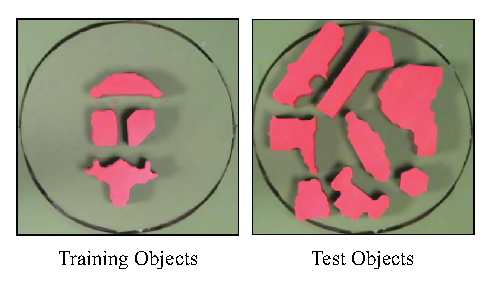
\includegraphics{f_figs/shapes_set.eps}

\caption{\footnotesize  The Training objects on the right are the four objects used in training. The test objects on the
left represent represent objects that were added in our test configurations. Every test configuration contained at least
one of the objects on the right.}

\label{fig:shape_set}
\end{figure}


\begin{figure}[t]
\centering
\includegraphics{f_figs/succes_measure.eps}

\caption{\footnotesize  Right: examples of training configurations we presented to the robot. The shapes were arranged
around the goal object in different poses and in different parts of the workspace. At test time, we considered similar configurations but 
added some unknown objects not present in the test set. }
\vspace*{-20pt}
\label{fig:suc_meas}
\end{figure}

\subsection{Experimental Setup}
For the grasping in clutter task, we consider objects made of Medium Density Fiberboard with an average 4" diameter and 3" in height. The objects used to form clutter are red extruded polygons while the goal object is a yellow cylinder.  The robot workspace, which is green, consists of a  30" disk region which is
surrounded by an elevated plate constraining the objects to a ring and prohibiting them from leaving the camera's field of view. 


To test the performance of each robot policy, we created a test set composed of 20 different configurations each containing
objects that were not in the training set.  The training objects and test
objects introduced during testing are shown in Fig. \ref{fig:shape_set}. The test set configurations varied by placing
test objects from Fig. \ref{fig:shape_set} with objects we trained on in similar configurations. Examples of training and test configurations are shown in Fig. \ref{fig:suc_meas}.  During training and testing, we manually place the objects in configurations. However, a hardware mechanism that moves the objects around, such as a pre-defined sweeping motion from the robot arm, could be used in future work. We measure success by whether the object was in the gripper at the final timestep. We define reliability or $\rho$ as the percentage of successful configurations.

Per iteration of Hierarchical DAgger, we collect 20 trajectories on different training configurations and then have a supervisor provide 20 demonstrations. We do this to sample a variety of configurations with the current policy before updating the weights. Thus 100 robotic trials correspond to 5 iterations of DAgger.

\subsection{Three Types of Supervisors}

\begin{figure*}[t]
\centering
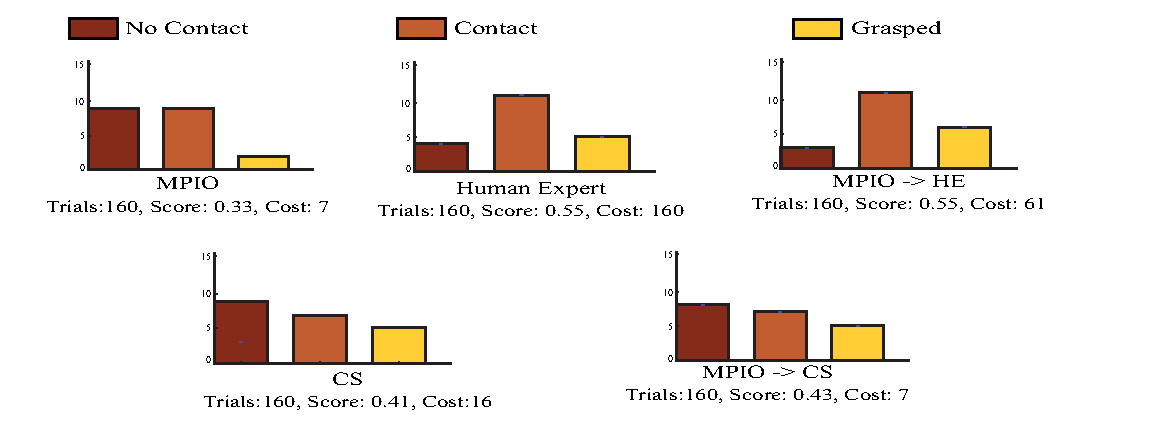
\includegraphics{f_figs/results.eps}

\caption{ \footnotesize The reliability or $\rho$, which is a measure of performance on previously unseen objects, of each policy trained with a supervisor is reported. The bar graphs
shows the number of successful and failed trials. The top row 
reports results for the MPIO ($\rho = 30\%$), Crowd-Sourced ($\rho = 35\%$) and  Expert ($\rho = 55\%$) supervisor in isolation.
The bottom  left and middle correspond to hierarchical supervisors: MPIO then Crowd-Sourced ($\rho = 45\%$) and MPIO then Expert ($\rho = 60\%$). All policies expect for the full hierarchy (bottom right) are trained on 160 demonstrations. The full hierarchy (bottom right)  has a fix budget of 160 Expert demonstrations, but  first leverages MPIO and Crowd-Sourced Supervisors until no improvement in reward from their demonstrations and is able to achieve a reliability of $\rho = 90\%$}
\vspace*{-20pt}
\label{fig:perf_results}
\end{figure*}

We first compare each supervisors' performance. We train the robot with MPIO Supervisor, Crowd-Sourced Supervisor or the Expert Supervisor for a fixed amount of 160 demonstrations on the training configurations. Our results shown in Fig. \ref{fig:perf_results}, show that for our fix budget of 160 trials the supervisors receive a reliability of $\rho = 30\%$, $\rho = 35\%$ and $\rho = 55\%$, respectively. 

When testing the Crowd-Sourced Supervisor, we hired  44 AMT workers. We found only
21 AMT workers were able to pass the quality check and continue providing demonstrations as described in Sec. \ref{sec:sys}. On average a worker would
provide 8 demonstrations before choosing to not provide any more. A single demonstrations would take 50s to provide.  

We are next interested in testing how the supervisors perform in the hierarchy. We divide the original budget of 160 demonstrations to 100 MPIO demonstrations and 60 demonstrations of a higher skill supervisor (i.e. Crowd-Sourced or Expert). The choice of 100 demonstrations was made due to no improvement in reward from the MPIO Supervisor after 100 demonstrations. 

Results shown in Fig. \ref{fig:perf_results}, suggest that a hierarchy of supervisor with MPIO and Crowd-Sourced achieves a reliability of $\rho = 45\%$ and MPIO and Expert achieves a reliability of $\rho = 60\%$. This suggests that a hierarchy of supervisors can be beneficial to increase reliability of a robot at a lower cost than only with an Expert Supervisor. 




\subsection{Full Hierarchy}
Given a fixed budget of 160 Expert Supervisor demonstrations, which achieves $55\%$ reliability,  we are interested in increasing relaibility by leveraging the less costly supervisors, MPIO and Crowd-Sourced.  We thus had MPIO and Crowd-Sourced supervisor provide demonstrations until we observed the reward achieved was not increasing. This results in the
MPIO Supervisors providing 100 demonstrations, the Crowd-Sourced Supervisor providing 120 demonstrations. We then had the Expert Supervisor provide a fix budget of 160 demonstrations. The resulting policy had a reliability of $90\%$ as shown in Fig. \ref{fig:perf_results}.

Investigating the learned policy, we observed that it appears to find gaps in between the clutter objects and sweeps
left to right,  until the objects are pushed apart and then moves towards the goal object, as illustrated in Fig.
\ref{fig:teaser}. We noticed that the magnitude of the sweeping motion appeared anti-proportional to the size of the gap in
 between the cluttered objects. For example, two cluttered objects placed close together in front of the goal object would  cause a high frequency of sweeping. While a single object in front of the goal object would often result in a single sweeping motion pushing the obstacle away from the goal object.  We also noticed that the robot would in general stop once it reached the goal object. However, it was rare to see the robot go backwards and correct itself, despite those demonstrations being given. 

 While our policy showed improved performance when trained using a hierarchy, failure modes persisted in our test
configurations. Common failure modes are either that the robot
sweeps too far and jams the objects against the inscribed circle around the workspace or a smaller obstacle object was caught in the gripper while being pushed.

\subsection{Advancing in the Hierarchy}
We lastly test how to advance between supervisors in the hierarchy. We examine the situation where the robot is first trained with the MPIO supervisor for 100 demonstrations and then the Expert Supervisor for 60 demonstrations. 

We are interested in testing the following strategies for changing supervisors 1) aggregating the two datasets of the demonstrations collected with both MPIO and Expert Supervisors 2)
transferring only the weights of the neural network policy or $\theta$  to initialize training with the Expert and not retraining on the MPIO Supervisor's demonstrations 3) transferring only the weights of the neural network policy but
adding the values output by $\pi_\theta(\bx)$  instead of $\tilde{\pi}_m(\bx)$ in the states visited that the
Expert Supervisor's demonstrations are similar too the output of the policy as measured by the following $||\tilde{\pi}_m(\bx) - \pi_\theta(\bx)||^2_2
< 0.01$. Thus, acting as a form of regularization on the optimization since stochastic gradient on a section of the mini-batch update would be zero for examples where the policy trained with the MPIO Supervisor matches that of the Expert. 

 Our results reported in Fig.\ref{fig:cost_result}, show that the aggregation strategy achieves reliability, $\rho=15\%$, the weight transfer strategy achieves $\rho = 60\%$ and the regularized stochastic gradient update strategy achieves $\rho=65\%$. Thus, suggesting that techniques to help the policy remain close to the previously trained supervisor are useful for effectively switching between supervisors.

\begin{figure}[t]
\centering 
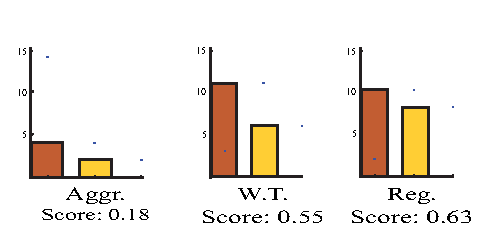
\includegraphics{f_figs/cost_result.eps}

\caption{\footnotesize The performance of each policy trained with a different data management strategy is reported. The
bar graph show the breakdown in terms of Failure and Success on the test configurations.Each policy was trained with the MPIO and then the Human Expert supervisor. From left to right , we display the following: Dataset Aggregation, Weight Transfer and Regularization. Regularization achieves the highest performing reliability of ($\rho = 0.65\%$) }

\label{fig:cost_result}
\vspace*{-22pt}
\end{figure}


\section{Discussions and Future Work}
Robot grasping in clutter is a challenging problem for automation in warehouse order assembly and home cleaning due to uncertainty arising from sensing and control and the inherent complexity of push mechanics. We introduce a version of the problem where a yellow cylinder must be grasped by a planar robot arm amid extruded objects with a variety of shapes and positions.  Results suggest that this task is amenable to a Learning from Demonstrations approach such as DAgger or SHIV but can put a burden on human experts.

To reduce the burden, we consider two alternative supervisors:  one is a motion planner that ignores obstacles (MPIO) and the second is crowd-sourced workers from Amazon Mechanical Turk who provide demonstrations using a novel overlay interface.  Results show as expected that the reliability of the policies depend on the skill level of the demonstrations.  We introduce a hierarchical approach where supervisors with differing skill levels are combined.  Results suggest that staging supervisors in terms of increasing skill level can bootstrap LfD to learn reliable policies, in this case the robot learns a counter-intuitive policy where the it sweeps the gripper back and forth to clear obstacles before grasping.

To our knowledge this is the first study of hierarchical supervisors for Learning from Demonstrations. In future work, we will perform more experiments in this context with added noise in perception and control, and study how the policies generalize to a broader variety of objects and different configurations. We will also study the comparative performance of other motion planning-based supervisors and study how hierarchical approaches can be applied to tasks such as driving and assembly.  Further information, video and code can be found at the following \url{http://berkeleyautomation.github.io/HierSupCASE/}. 




 \section{Acknowledgments} 
This research was performed in UC Berkeley's Automation Sciences Lab under the UC Berkeley Center for Information Technology in the Interest of Society (CITRIS) "People and Robots" Initiative. This work is supported in part by the U.S. National Science Foundation under Award IIS-1227536, NSF-Graduate Research Fellowship, by the Knut and Alice Wallenberg Foundation and the National Defense Science and Engineering Graduate Fellowship Program. We thank Steve McKinely and Meng Guo for help in building the hardware setup.  

  
\bibliographystyle{IEEEtranS}
\bibliography{references}



\end{document}
%\subsection{Hierarchies} If the robot could learn the policy  perfectly, this state density would match the one encountered in user examples. But if the robot makes an error, that error changes the distribution of states that the robot will visit, which can lead to states that are far away from any examples and difficult to generalize to~\cite{pomerleau1989alvinn}. This motivates iterative algorithms like DAgger, which iterate between learning a policy and the supervisor providing examples. We  introduce the concept of their being a set of supervisors each with an associated cost and skill level. Denote $\tilde{\pi}_M$ the most skilled and costly supervisor in this set. This supervisor could for example be a person with a Phd in machine learning and robotics. We formally define how each supervisor in the set is related to each other in Sec. \ref{sec:hS}.  Every time a supervisor is queried a cost, $C_m$, is incurred this could be an hourly pay rate or computational time. While Eq. \ref{eq:LFD_obj} is the primary objective of our algorithm a secondary objective is to reduce the cumulative cost associated with training the robot. Thus, we are interested in solving the following objective

%where $J$ is the number of queries need to satisfy the constraint on expected surrogate loss, $C_{m,j}$ denotes the cost incurred by querying the supervisor at that iteration and $\epsilon$ is a user-defined threshold on how close robot policy is to match the highest quality supervisor. We present our algorithm, LEATHERMAN, which aims to solve Eq. \ref{eq:bugjet_LFD_obj}.
 

%\subsection{Hierarchy of Supervisors}\label{sec:hS} Instead of one  supervisor,we propose a hierarchy  of $M$ supervisors where for each supervisor $\tilde{\pi}_m$, there is an associated expected cumulative reward $R_m = \int \sum^T_{t=1} r(\mathbf{x}_t, \tilde{\pi}_m(x)) p(\tau |\tilde{\pi}_m)d\tau$, where $p(\tau |\tilde{\pi}_m)$ denotes the average distribution of states the supervisor encounters. We also denote some measure of cost $C_m$ that is ascribed to the supervisor, such as computational time or monetary expense. Generally the rank of supervisors in terms of cost is equivalent to the rank of supervisor in the terms of expected cumulative reward. Thus, the least costly supervisor will receive the lowest expected cumulative reward. 

%Additionally for two supervisors $\tilde{\pi}_m$ and $\tilde{\pi}_{m+1}$ to be in the hierarchy, they must only disagree in expectation on a subset of the work space to some precision $\tilde{\epsilon}$. Denote the set of states two supervisors disagree as $\mathcal{X}_{m,m+1} = \lbrace \mathbf{x} | ||\tilde{\pi}_m(\mathbf{x}) - \tilde{\pi}_{m+1}(\mathbf{x}) ||^2_2 > \tilde{\epsilon} \rbrace$ .We enforce the condition $\mathcal{X}_{m,m+1} \subset \mathcal{X}$ because if two supervisors never provided the same examples then all states would have to be relabeled by the next supervisor in the hierarchy. 

%We formally define an ordering on supervisors:

%\begin{definition} Two supervisors $\tilde{\pi}_m$ and $\tilde{\pi}_{m+1}$ are in a hierarchy if  $C_m < C_{m+1}$  and  $\mathcal{X}_{m,m+1} \subset \mathcal{X}$ \end{definition}

%Violation of this definition could result in no additional benefit from the LEATHERMAN algorithm or potentially worst a higher budget incurred than without using a hierarchy of supervisors.
